%% LyX 2.3.6.1 created this file.  For more info, see http://www.lyx.org/.
%% Do not edit unless you really know what you are doing.
\documentclass[english,british]{article}
\usepackage[T1]{fontenc}
\usepackage[latin9]{inputenc}
\usepackage{geometry}
\geometry{verbose,tmargin=2cm,bmargin=2cm,lmargin=1cm,rmargin=1cm}
\usepackage{babel}
\usepackage{float}
\usepackage{amsmath}
\usepackage{amsthm}
\usepackage{amssymb}
\usepackage{graphicx}
\usepackage{setspace}
\doublespacing
\usepackage[unicode=true]
 {hyperref}

\makeatletter
%%%%%%%%%%%%%%%%%%%%%%%%%%%%%% User specified LaTeX commands.
\usepackage{indentfirst}
\usepackage{mathtools}

\makeatother

\begin{document}
\title{Study of liquid and nematic phases in hard spherocylinders}
\author{Leonardo H�gens and Johanna L�mker}
\maketitle
\begin{abstract}
In this project we studied a system of hard spherocylinders using
NVT and NPT Monte Carlo msimulations. We used the paper \emph{Tracing
the phase boundaries of hard spherocylinders }(Bolhuis and Frenkel,
1997) as a reference, trying to replicate some of its results. What
we found was that (...)
\end{abstract}

\section{Introduction}

The model we study in this project is the hard spherocylinders model,
and the interest in their study comes from their capability to form
all sorts of order phases, each of them mainly characterized by order/disorder
in their position and orientation, e.g. the liquid phase is the most
disordered and isotropic, while in the solid phase every spherocylinder
shares the same orientation, and they are positioned in layers orthogonal
to theirs orientation. 

The main reference we used to compare our results to was \emph{Tracing
the phase boundaries of hard spherocylinders }(Bolhuis and Frenkel,
1997) \cite{paper1}. Our first goal was to use Monte Carlo NVT simulations
to observe some of the phases of the hard spherocylinders, mainly
the liquid and nematic ones, and checking if their existence with
the used parameters makes sense according to the phase diagrams present
in \cite{paper1}. Our second goal was to use NPT Monte Carlo simulations
to build an volume-pressure state curve, as the paper has several
of them for us to compare with. During these simulations, we pay close
attention to the nematic order parameter $S$, which we'll define
later, that measures whether or not the spherocylinders have an overall
common orientation.

\section{Model}

The model we study in this project is the hard spherocylinder model,
which consists of $N$ cylinders of length $L$ that have half spheres
of diameter $D$ attached to each of its ends, whose interaction potential
is infinite if there is an overlap or touch between two of them and
vanished if there are no overlaps. The volume of a spherocylinder
is thus 
\[
v_{0}=\pi\left(\frac{LD^{2}}{4}+\frac{D^{3}}{6}\right).
\]

The particles are contained in a box of volume $V$ with periodic
boundary conditions. The convention used in \cite{paper1} and which
we'll use for the density in our project will be to use the reduced
density $\rho^{*}$, defined as 
\[
\rho^{*}=\frac{\rho}{\rho_{\text{cp}}},
\]

where $\rho_{\text{cp}}=\frac{2}{\sqrt{2}+\left(L/D\right)\sqrt{3}}$
and 
\[
\rho=\frac{Nv_{0}}{V}.
\]

To measure the orientation order/disorder of the system, we'll refer
to the nematic order parameter $S$, defined by 
\[
S=\frac{1}{N}\sum_{i=1}^{N}\left[\frac{3}{2}\cos^{2}\left(\theta_{i}\right)-\frac{1}{2}\right]
\]

where $\theta_{i}$ is the angle formed by the orientation vector
of particle $i$, $\boldsymbol{n}_{i}$, and the \emph{director} vector
$\boldsymbol{n}_{d}$, which is the normalized average of all the
orientation vectors, so:
\[
\cos\left(\theta_{i}\right)=\boldsymbol{n}_{i}\cdot\boldsymbol{n}_{d}=\boldsymbol{n}_{i}\cdot\frac{\sum_{j=1}^{N}\boldsymbol{n}_{j}}{\left|\left|\sum_{j=1}^{N}\boldsymbol{n}_{j}\right|\right|}
\]

In the case where all the particles have that same orientation, i.e.
$\boldsymbol{n}_{i}=\boldsymbol{n}\,\,\forall\,i$, we have $\cos\theta=1$,
which implies $S=1$. 

In the NPT simulations, we'll use the quantity $\beta Pv_{0}$ as
a proxy for the pressure $P$, and temperature $\beta$. The quantity
$\frac{L}{D}$ is also referred to as shape anisotropy, the limit
$\frac{L}{D}=0$ corresponds to regular spheres of diameter $D$,
and the limit $\frac{L}{D}\rightarrow+\infty$ corresponds to 1-dimensional
rods of length $L$.

\section{Methods}

\subsection{Minimum distance between $\left(L,D\right)$ spherocylinders}

To perform our simulations, we need to be able to check for overlapping
spherocylinders in a numeric way. To this end, we implemented the
algorithm described in \emph{A fast algorithm to evaluate the shortest
distance between rods }(Vega and Lago, 1994) \cite{paper2}. The minimum
distance this algorithm returns refers two one dimensional (thick-less)
rods, and thus two spherocylinders overlap if this distance is equal
or less than $D$.

\subsection{Visualization}

In order to observe qualitatively the phase of the system during a
simulation, we used the program \emph{Viscol}, publicly accessible
via \href{https://webspace.science.uu.nl/~herme107/viscol/}{https://webspace.science.uu.nl/~herme107/viscol/}.
In our simulation, we store each particle's position $\boldsymbol{r}_{i}$
and orientation vector $\boldsymbol{n}_{i}$, but unfortunately the
input format required by the program for it to plot the particles
is not simply the $6$ values of those two vectors. Instead, it is
required to build a rotation matrix $M$, in the picture where the
matrix acts on the frame in which the particle is fixed, and not on
the particle itself. Plugging in the identity matrix, the particle
was oriented in the $\hat{z}$ direction, which means that $M$ is
given by:
\begin{align*}
M & =R_{y}\left(-\theta\right)R_{z}\left(\phi\right)\\
 & =\left(\begin{array}{llc}
\cos\theta & 0 & -\sin\theta\\
0 & 1 & 0\\
\sin\theta & 0 & \cos\theta
\end{array}\right)\left(\begin{array}{llc}
\cos\phi & \sin\phi & 0\\
-\sin\phi & \cos\phi & 0\\
0 & 0 & 1
\end{array}\right)\\
 & =\left(\begin{array}{llc}
\cos\theta\cos\phi & \cos\theta\sin\phi & -\sin\theta\\
-\sin\phi & \cos\phi & 0\\
\sin\theta\cos\phi & \sin\theta\sin\phi & \cos\theta
\end{array}\right)
\end{align*}

where for a given orientation vector $\boldsymbol{n}$ we can determine
the elements of this matrix as follows:
\begin{align*}
\cos\theta & =\boldsymbol{n}\cdot\hat{z}\\
\sin\theta & =\sqrt{n_{x}^{2}+n_{y}^{2}}\\
\cos\phi & =\frac{n_{x}}{\sin\theta}\\
\sin\phi & =\frac{n_{y}}{\sin\theta}
\end{align*}


\subsection{NVT Monte Carlo}

To perform an NVT Monte Carlo simulation, we first pick an initial
configuration of the system, i.e. $N$ positions and orientation vectors
with no existent overlap. One initial configuration that is straightforward
to build is that of an FCC grid, for which no overlaps will exists
\emph{a priori}, and thus it is very convenient to use. In the course
of our project we did a lot of simulations, and the saved configurations
generated in NVT or NPT runs are also very convenient to use, specially
because they (the ones we studied) are mostly liquid and ranging various
densities, which if we wanted to artificially generate one liquid
configuration at a specific density it would most likely involve a
lot of inefficient trial and error. 

At each NVT MC step we pick one particle with uniform probability,
and propose to either change is position or orientation slightly,
also with uniform probability. If this displacement does not cause
the chosen particle to overlap one of its neighboring particles, we
accept it with probability of one, since the Metropolis acceptance
weight is given by
\[
\frac{\operatorname{acc}(\text{old}\rightarrow\text{new})}{\operatorname{acc}(\text{new}\rightarrow\text{old})}=\exp\left[-\beta\left(U\left(\mathbf{s}^{N};L^{\prime}\right)-U\left(\mathbf{s}^{N};L\right)+P\left(V^{\prime}-V\right)-N\beta^{-1}\ln\left(V^{\prime}/V\right)\right)\right]
\]

where in our case the hard particle interaction potential $U$ makes
this acceptance ratio always $1$ in the absence of overlaps and $0$
in their presence, and in NVT the volume $V$ is kept constant.

\subsection{NPT Monte Carlo}

An NPT MC simulation differs from an NVT one in the following manner:
at each step of the simulation, we propose to change the volume of
the box containing the particles with probability $\mathbb{\mathbb{P}}_{\text{vol}}$,
by scaling the box boundaries and positions of the particles. If a
generated uniformly random number is less than $\mathbb{\mathbb{P}}_{\text{vol}}$,
we propose that scaling, otherwise a regular NVT step will be performed.
After rejecting the proposal in the case where it has overlaps, we
accept the proposal according to the probability:
\[
\frac{\operatorname{acc}(o\rightarrow n)}{\operatorname{acc}(n\rightarrow o)}=\exp\left[-\beta P\left(V^{\prime}-V\right)+N\ln\left(V^{\prime}/V\right)\right]
\]


\section{Results and Discussions}

\subsection{NVT}

In our reference paper \cite{paper1}, a full phase diagram $\rho^{*}$
vs $\frac{L}{D}$ for $0<\frac{L}{D}<5$ is achieved, and it's represented
in the following Figure \ref{fig:phases}. Firstly, we implemented
and ran NVT simulations for fixed values of $\frac{L}{D}$ and $\rho^{*}$,
to then visualize equilibrium configurations and qualitatively assess
in which phase they are in, while also checking the nematic order
parameter $S$. 
\begin{figure}[H]
\begin{centering}
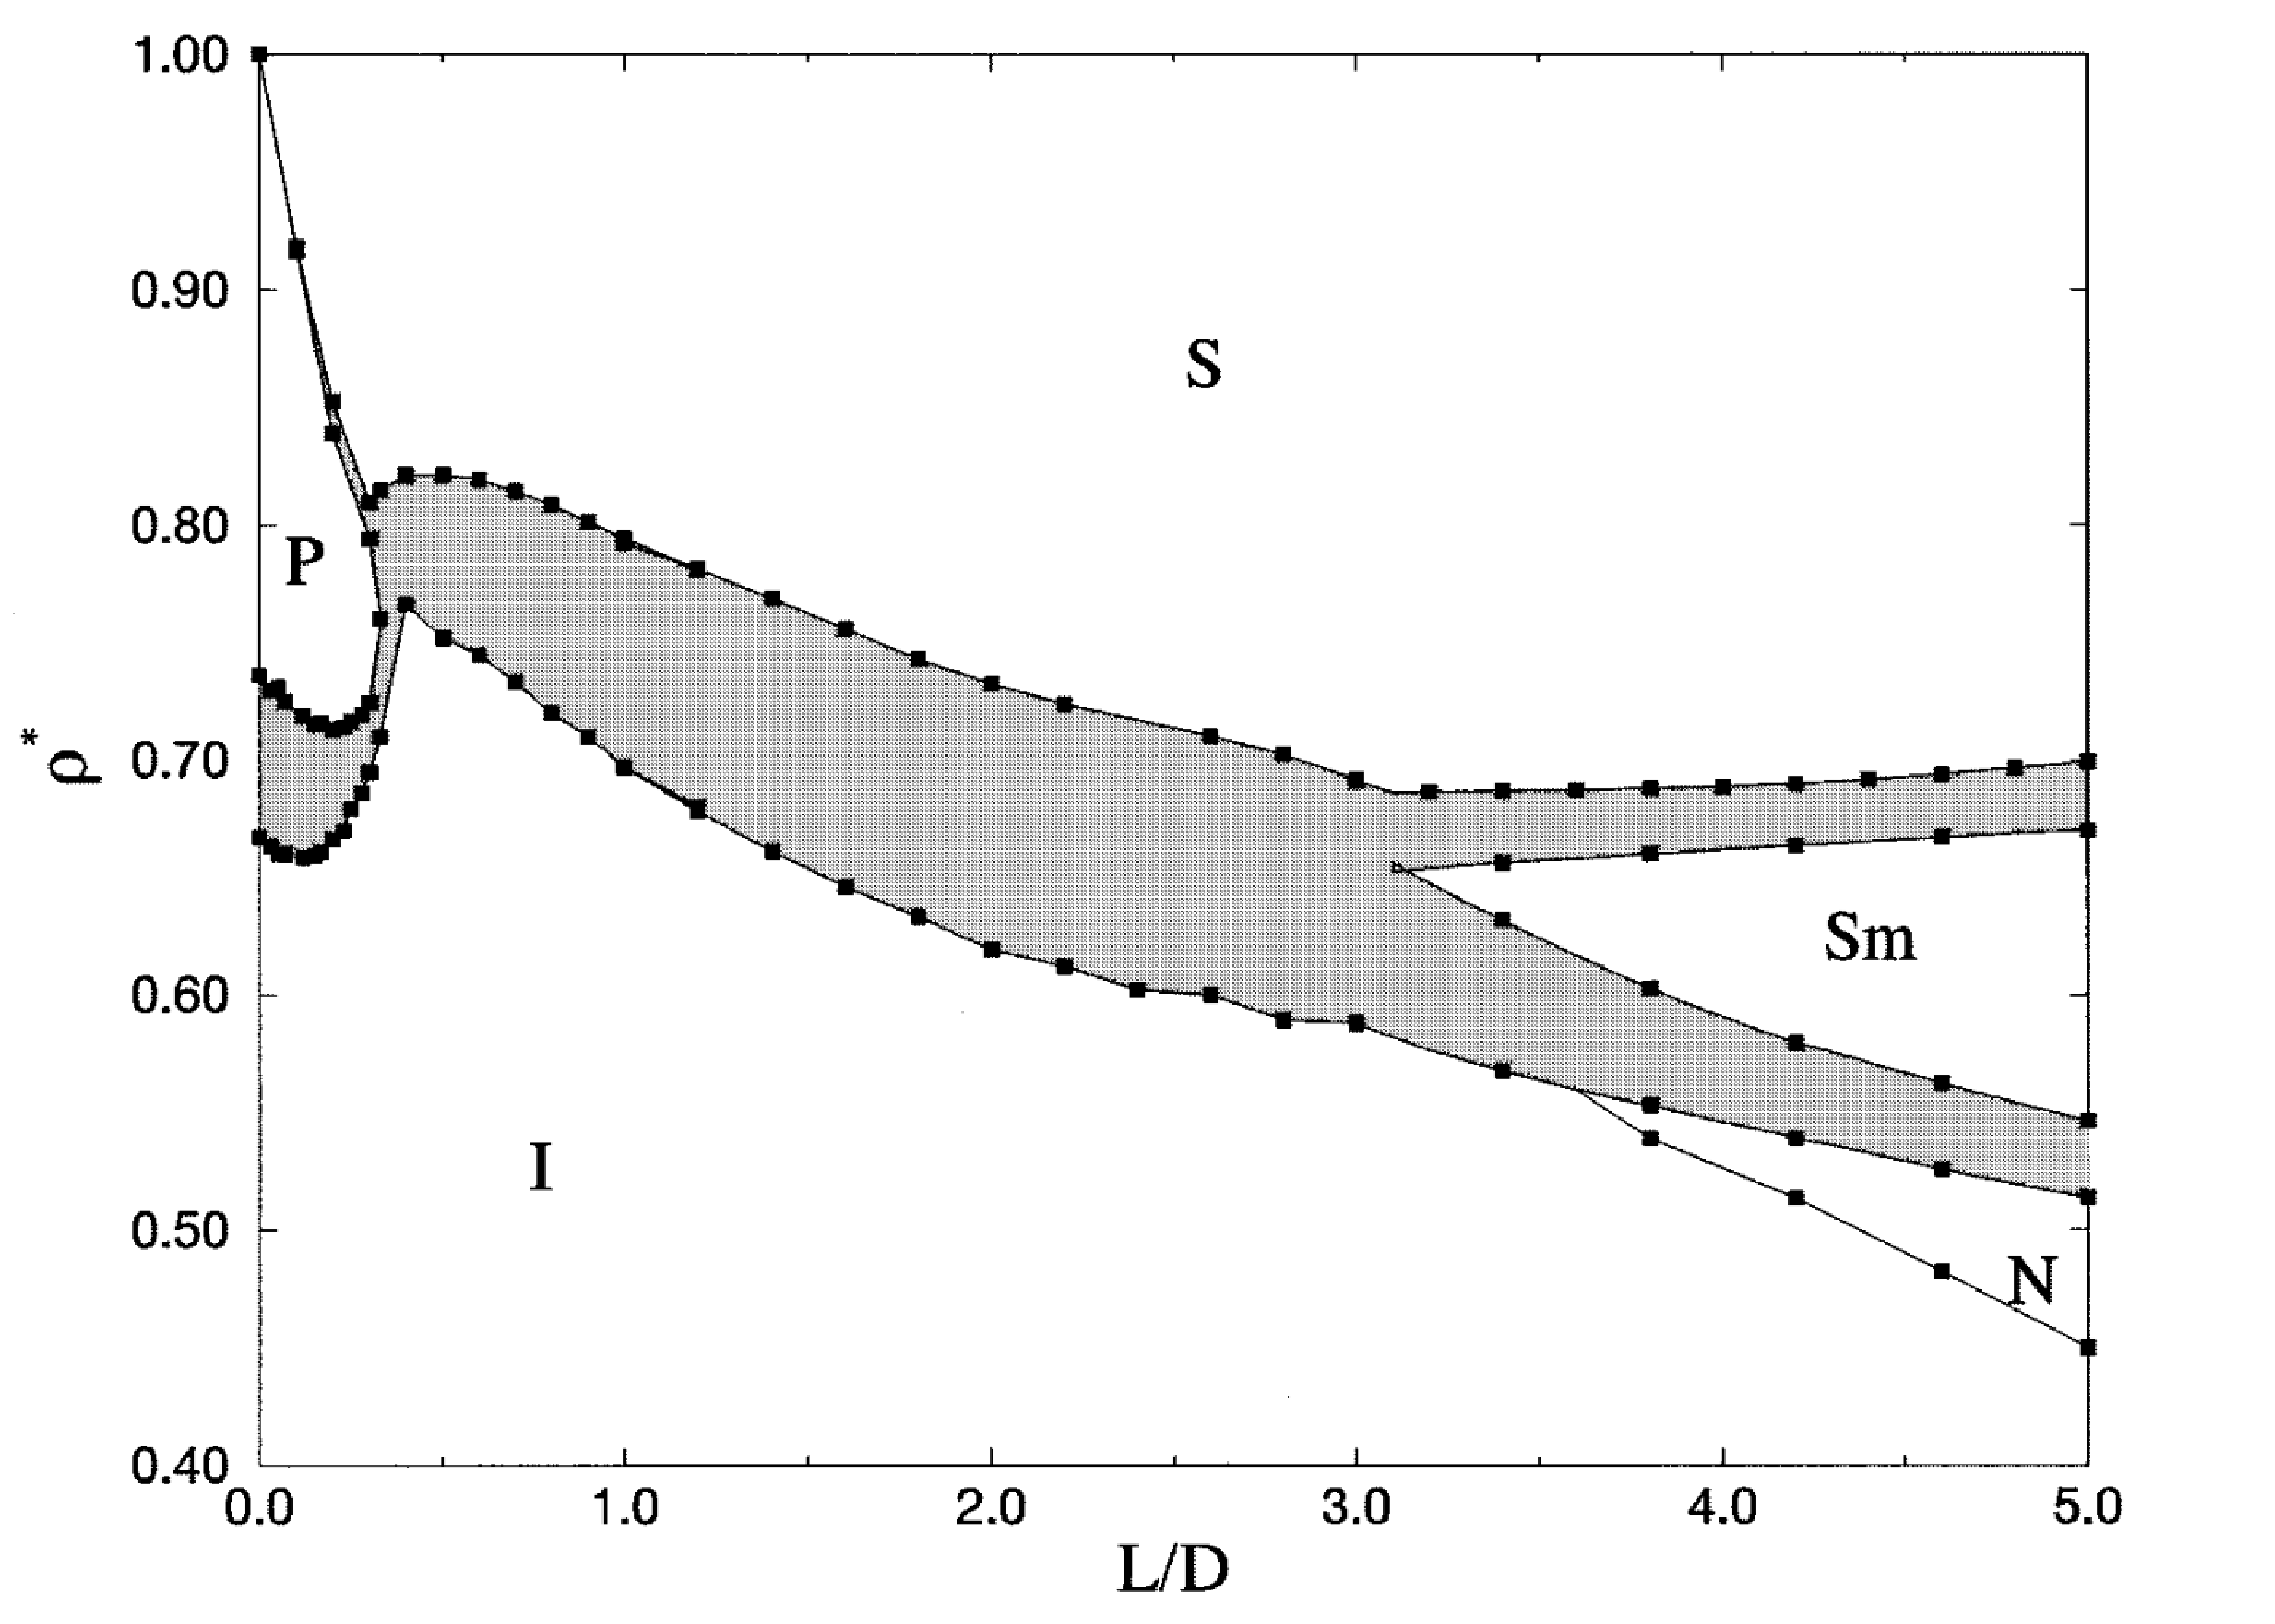
\includegraphics[width=0.8\textwidth]{/home/hugens/shared/uni/modsim/modsim/project/figures/phases}
\par\end{centering}
\caption{Phase diagram for hard spherocylinders.\label{fig:phases}}
\end{figure}

The convenient FCC configuration we usually started with to perform
these NVT simulations is represented below in Figure \ref{fig:fcc}.
At first we had some trouble with this since we were trying to use
a strictly cubic box, as it usually fixed, and that would result in
overlapping even for medium densities $\rho^{*}$. We fixed this issue
by only performing the scaling in the $x$ and $y$ directions to
achieve the desired density. We also left a few `leftover' space
along 3 of the faces of the box, as visible in Figure \ref{fig:fcc},
because if we filled the box entirely the particles in opposite faces
would effectively be in the same positions due to the periodic boundary
conditions, overlapping. 

\begin{figure}[H]
\begin{centering}
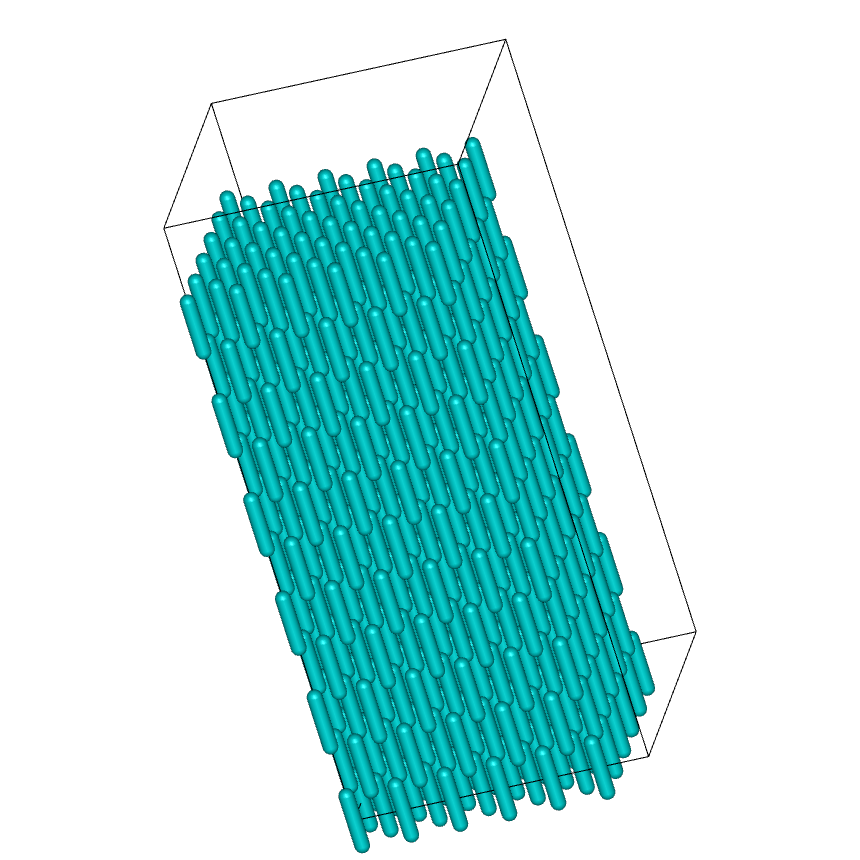
\includegraphics[width=0.3\textheight]{/home/hugens/shared/uni/modsim/modsim/project/figures/fcc}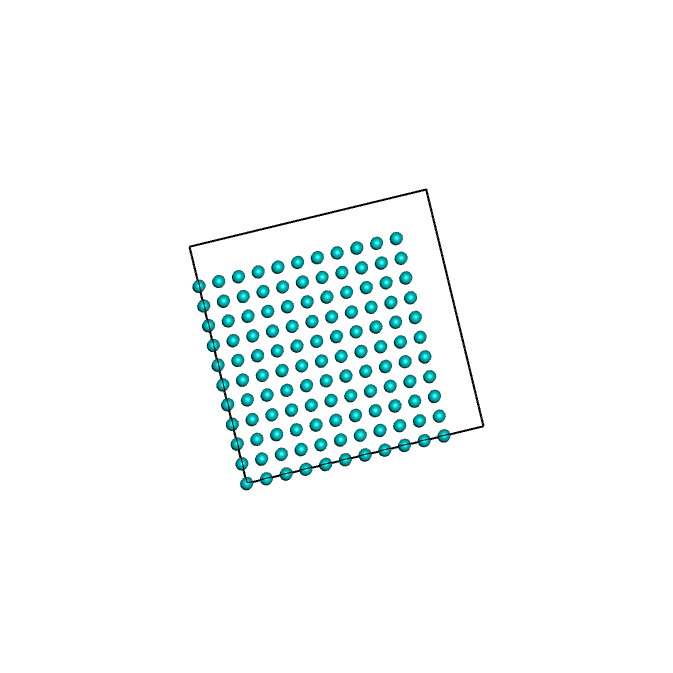
\includegraphics[width=0.3\textheight]{/home/hugens/shared/uni/modsim/modsim/project/figures/fcc_top}
\par\end{centering}
\caption{Initial FCC configurations.\label{fig:fcc}}
\end{figure}

The results we obtained are represented in the following Figure \ref{fig:our_phases}.
\begin{figure}[H]
\begin{centering}
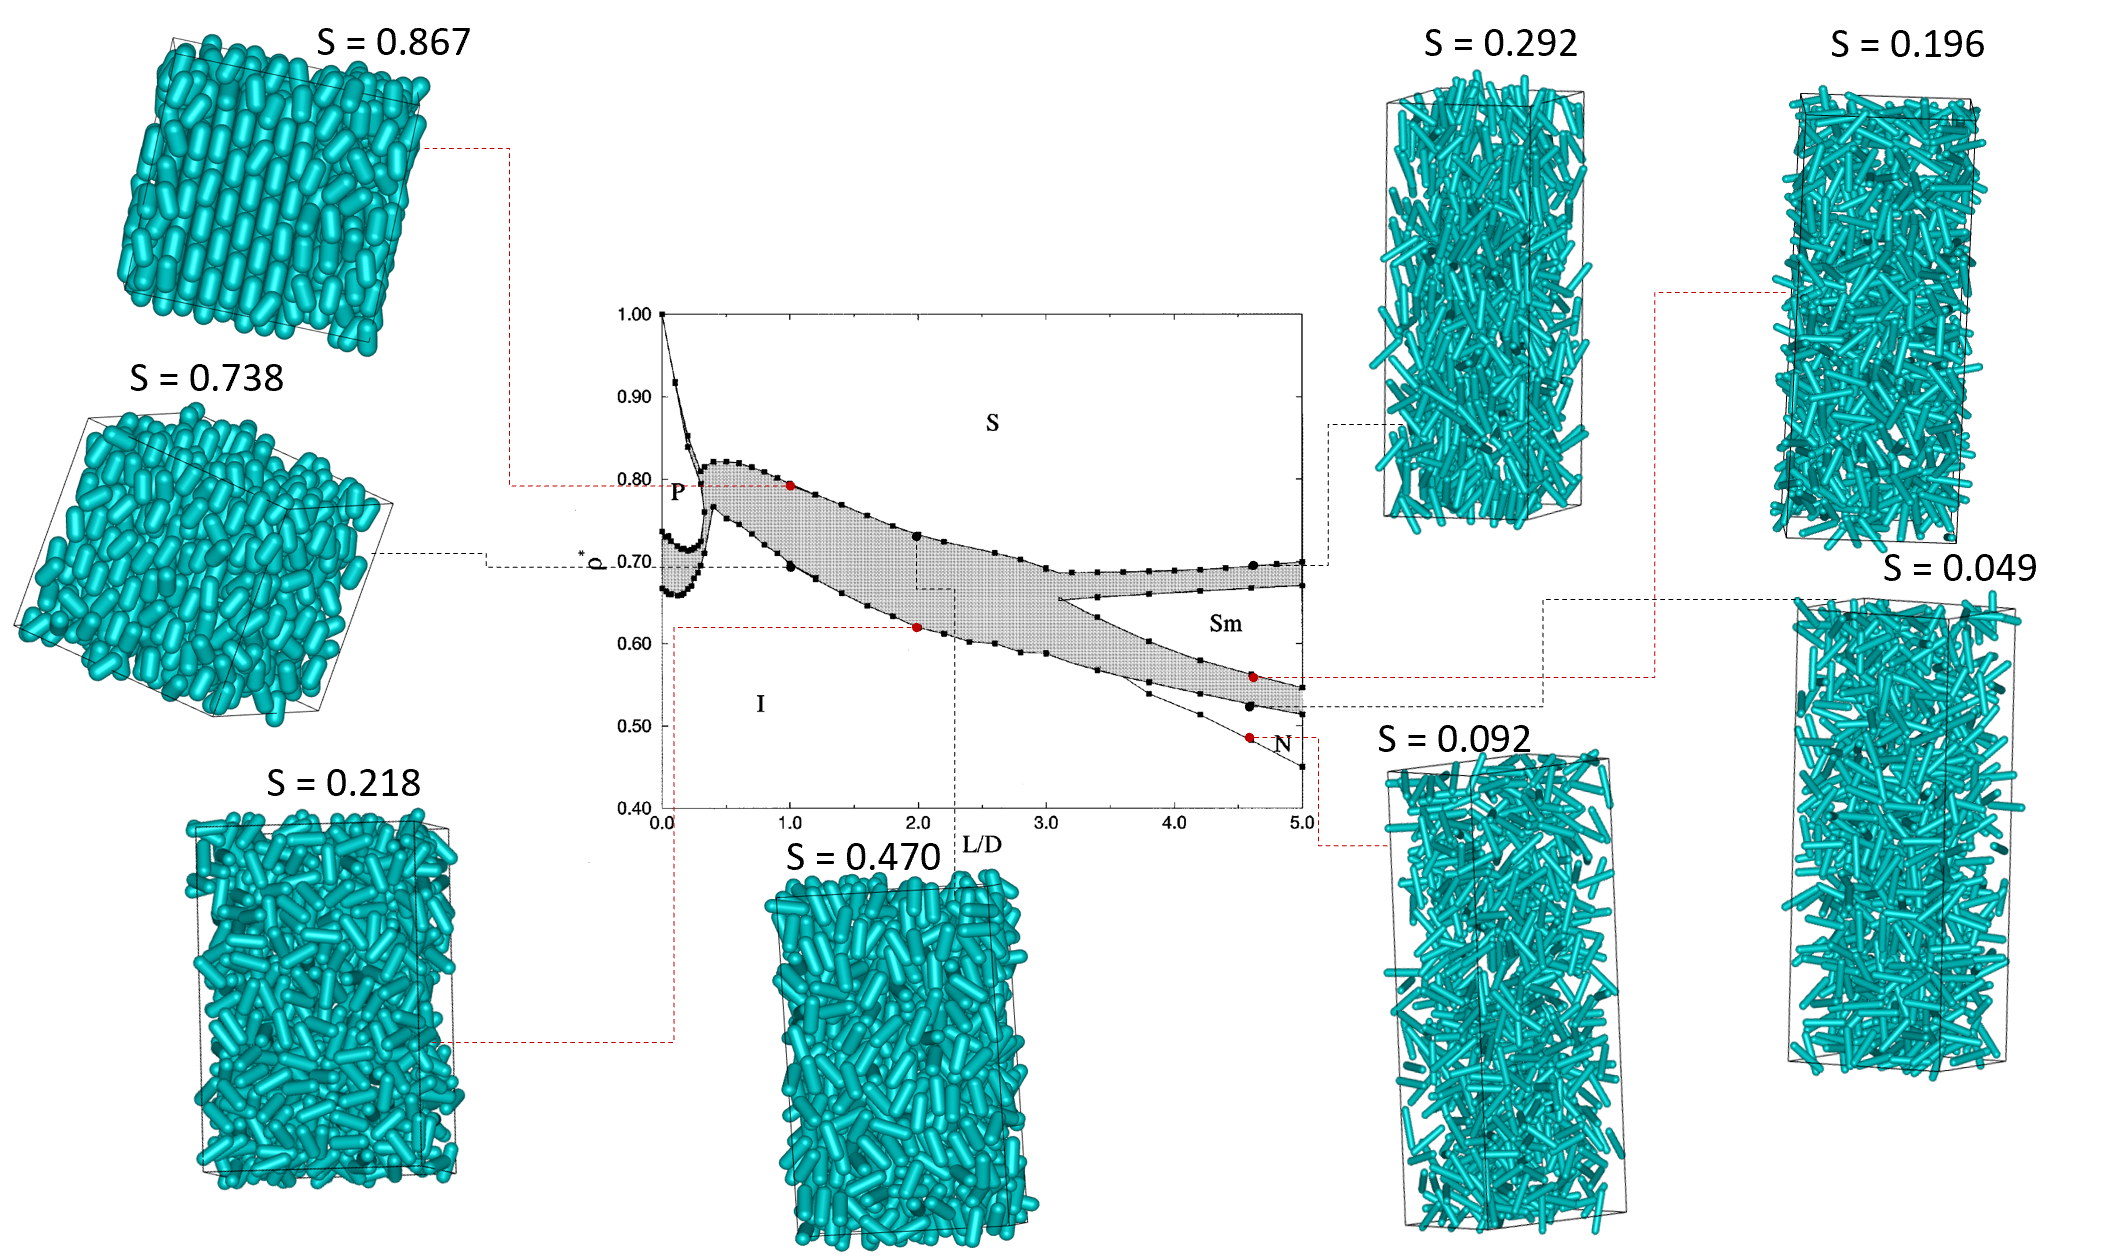
\includegraphics[width=0.8\textwidth]{/home/hugens/shared/uni/modsim/modsim/project/figures/model_configs}
\par\end{centering}
\caption{Visual representation of equilibrium configurations obtained using
NVT runs.\label{fig:our_phases}}
\end{figure}

In the represented equilibrium configurations, it seems like only
the one with $S=0.738$ could be argued not to be a liquid phase,
because of the high nematic order parameter. For the rest of the configurations,
from the low $S$ values and from a qualitative judgment of their
appearance, we may conclude they are all in the liquid phase. Below,
in Figure \ref{fig:phases_pic}, we present a figure taken from \cite{paper3},
in which several phases for hard cylinders are represented. Even though
these are not spherocylinders, these phases are also found in hard
spherocylinders. We think that a valid reason as to why basically
all of our configurations are liquid after NVT runs is that the usual
crystal phase for hard spherocylinders is characterized by hexagonally
ordered layers which are stacked in an 'AAA' fashion \cite{paper1},
and none are FCC-like configurations as represented in Figure \ref{fig:fcc},
i.e. it is possible that if we started from a configuration, e.g.
smectic B as in Figure \ref{fig:phases_pic}, the system could not
be able to melt (for a $\rho^{*}$ and $\frac{L}{D}$ values in the
appropriate region of the phase diagram \ref{fig:phases}).
\begin{figure}[H]
\begin{centering}
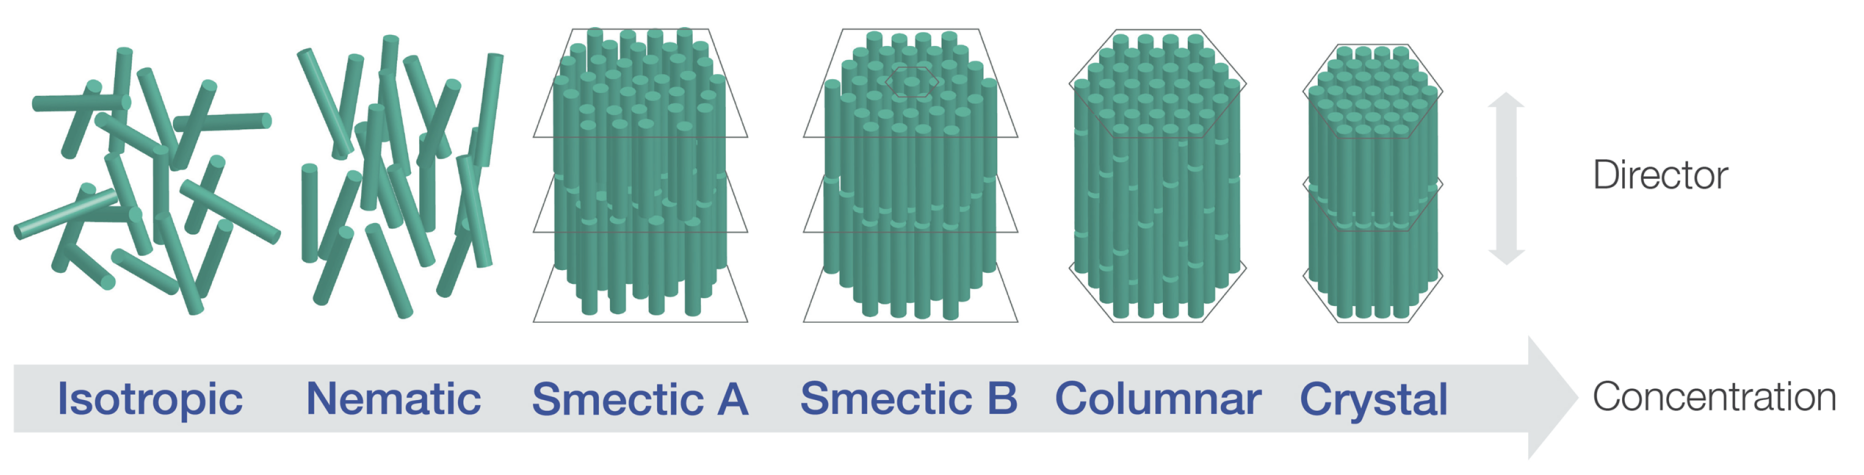
\includegraphics[width=1\textwidth]{/home/hugens/shared/uni/modsim/modsim/project/figures/phases_picture}
\par\end{centering}
\caption{Representation of some phases for hard cylinders.\label{fig:phases_pic}}
\end{figure}


\subsection{NPT}

In the reference paper \cite{paper1} there are several plots with
equations of state $\left(\rho^{*},\beta Pv_{0}\right)$ for various
shape anisotropy values. Since they are the liquid phase in these
plots does not suffer appreciable change among all the anisotropy
values, we decided to pick $L/D=3$ and try to replicate that plot,
represented in Figure \ref{fig:their_npt}.

\begin{figure}[H]
\begin{centering}
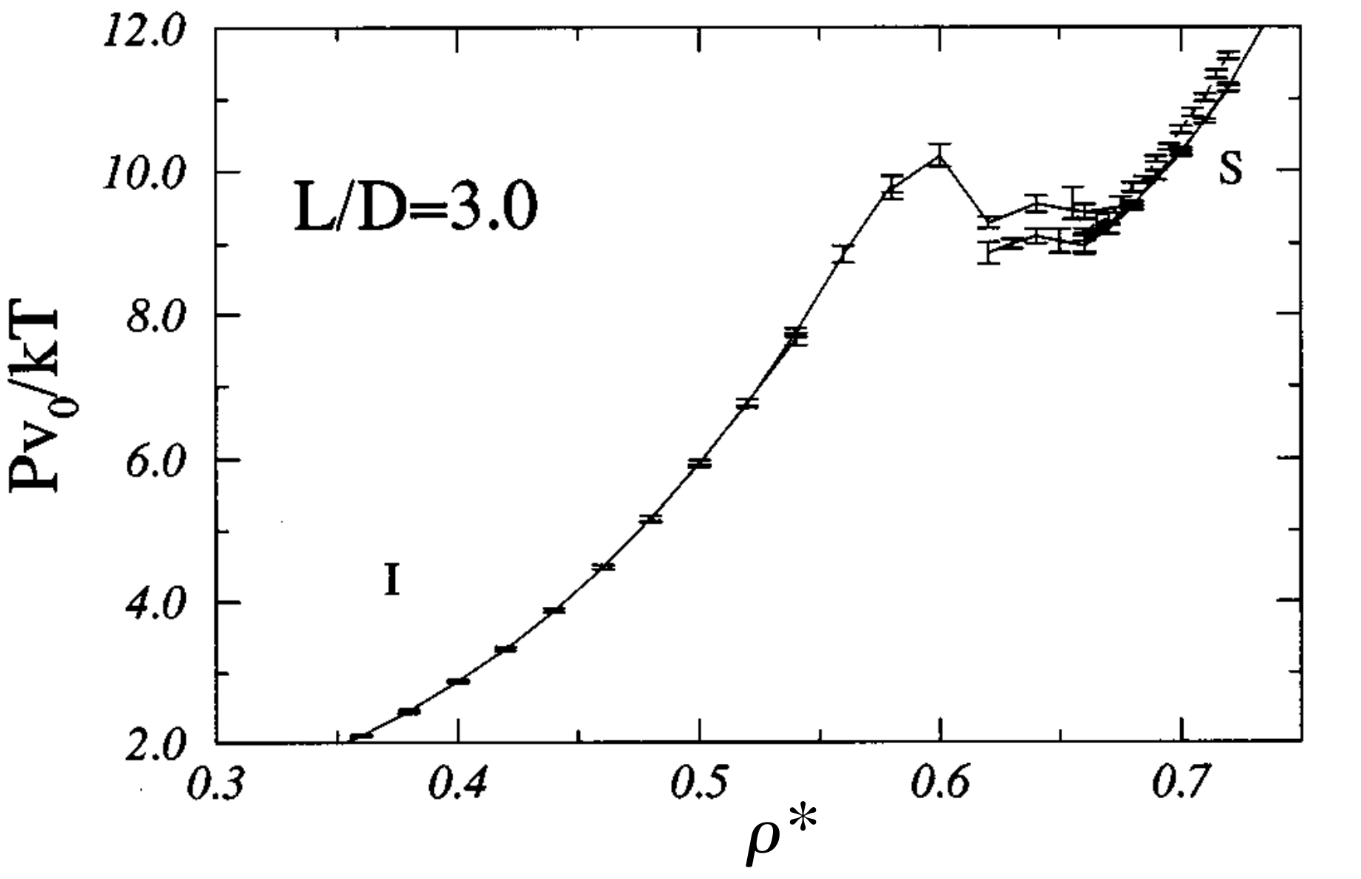
\includegraphics[width=0.7\textwidth]{/home/hugens/shared/uni/modsim/modsim/project/figures/their_npt}
\par\end{centering}
\caption{Equation of state for spherocylinders with shape anisotropy $L/D$
of 3. \label{fig:their_npt}}
\end{figure}

To this intent, we started with the value $\beta Pv_{0}=2$, with
a liquid initial configuration at $\rho^{*}=0.37$, which is already
pretty close to the equilibrium value. The maximum displacement values
we used were: for volume $dV=10$, for each component of position
$dl=0.01$, for each component of the orientation vector $dn=0.1$
(we always normalized the vector after the proposal), and $\mathbb{P}_{\text{vol}}=0.1$.
The reason we used these values is because we performed a few thousand
MC steps across several values of each displacement, and among the
ones that maximized the acceptance ratio these seemed the most reasonable,
given that all of them are quite small compared to the typical values
which they displace, and a small $\mathbb{P}_{\text{vol}}$ value
is expected to give the system room to adjust before it suffers contractions.
What we've observed is represented in Figure \ref{fig:NPT2}. During
the first half a million MC steps, the system appears to become `locked'
in a semi-ordered level of $S=0.6$, and the density $\rho^{*}$ appears
to slowly increase indefinitely.
\begin{figure}[H]
\begin{centering}
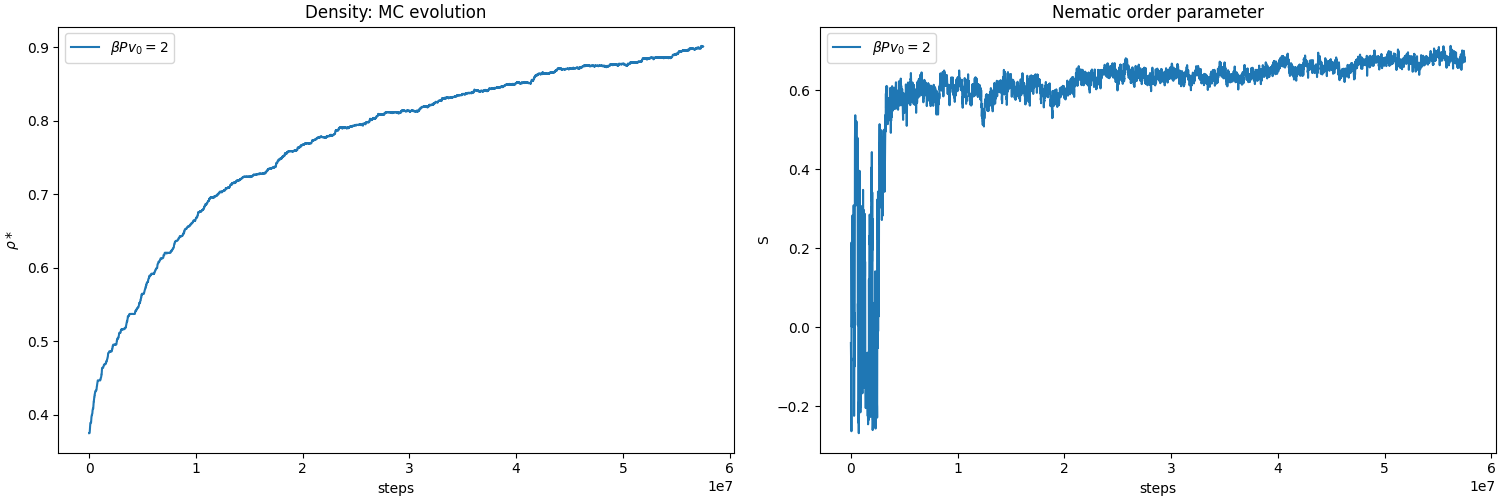
\includegraphics[width=1\textwidth]{/home/hugens/shared/uni/modsim/modsim/project/figures/NPT2}
\par\end{centering}
\caption{Left: Density evolution during a NPT run for $\beta Pv_{0}=2$. Right:
Nematic order parameter $S$ during the same run. \label{fig:NPT2}}
\end{figure}

To investigate this issue, we looked into the acceptance criteria
that follows the check for overlaps, i.e. if a proposed configuration
does not result in an overlap, the acceptance probability of proposed
change in volume $dV$ is:
\[
\text{acc}\left(dV\right)=\min\left\{ 1,\exp\left[-\beta PdV+N\ln\left(1+\frac{dV}{V}\right)\right]\right\} 
\]

Thus, we firstly looked at the maximum and minimum volume values of
the $\beta Pv_{0}=2$ run mentioned before, through plotting the volume
evolution of the run, represented in the following Figure \ref{fig:NPT2_vol}:
\begin{figure}[H]
\begin{centering}
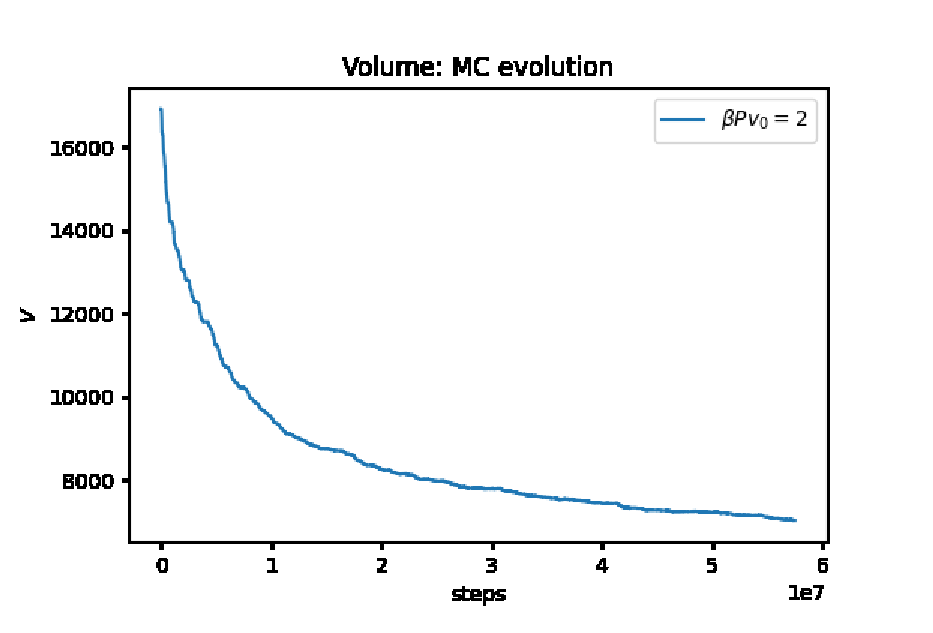
\includegraphics[width=0.5\textwidth]{/home/hugens/shared/uni/modsim/modsim/project/figures/vs}
\par\end{centering}
\caption{Volume evolution during a NPT run for $\beta Pv_{0}=2$ \label{fig:NPT2_vol}}
\end{figure}

Identifying $V_{\text{min}}\approx7000$ and $V_{\text{max}}\approx1600$,
we plotted the acceptance rate $\text{acc}\left(dV\right)$ for this
two values and several $\beta Pv_{0}$ values, and the results are
represented in the following Figure \ref{fig:acc}.
\begin{figure}[H]
\begin{centering}
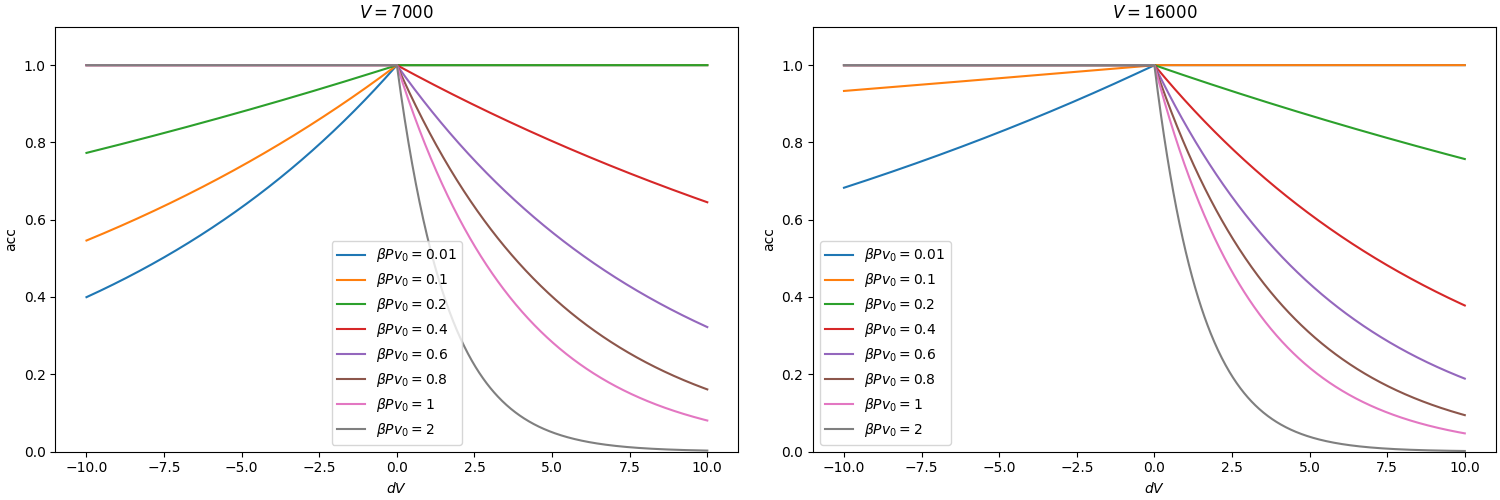
\includegraphics[width=1\textwidth]{/home/hugens/shared/uni/modsim/modsim/project/figures/acc}
\par\end{centering}
\caption{Acceptance criteria (after non-overlap check) for extreme volumes
and typical $\beta Pv_{0}$values. \label{fig:acc}}
\end{figure}

What we observe is that for values of the pressure such that $\beta Pv_{0}>1$,
proposed moves that decrease the volume $V$ are always accepted across
all the possibly reasonable $V$ values (since we tested with $V_{\min}$
and $V_{\max}$), while proposed moves that increase it are very rarely
accepted. Since we let the system explore a lot of configurations
before compressing ($\mathbb{P}_{\text{vol}}=0.1$), the behavior
we see in Figure \ref{fig:NPT2_vol} makes sense, even though it does
not agree with the reference paper \cite{paper1}, where the system
equilibrates at $\rho^{*}\approx0.37$. It is also intuitive that
even for $\beta Pv_{0}$ values for which there is always this biased
behavior towards decreasing the volume, at some point the spherocylinders
should get so close that almost any positional and orientational proposed
displacement would result in overlaps, but our results indicate that
this does not happen already pretty early in the $\beta Pv_{0}$ scale
of the paper, thus contradicting it. 

Based on the acceptance results we found (Figure \ref{fig:acc}),
we decided to run NPT simulations on $\beta Pv_{0}$ values that don't
seem to have this bias towards volume decreasing. Our results are
represented in the following Figure \ref{fig:NPT}.

\begin{figure}[H]
\begin{centering}
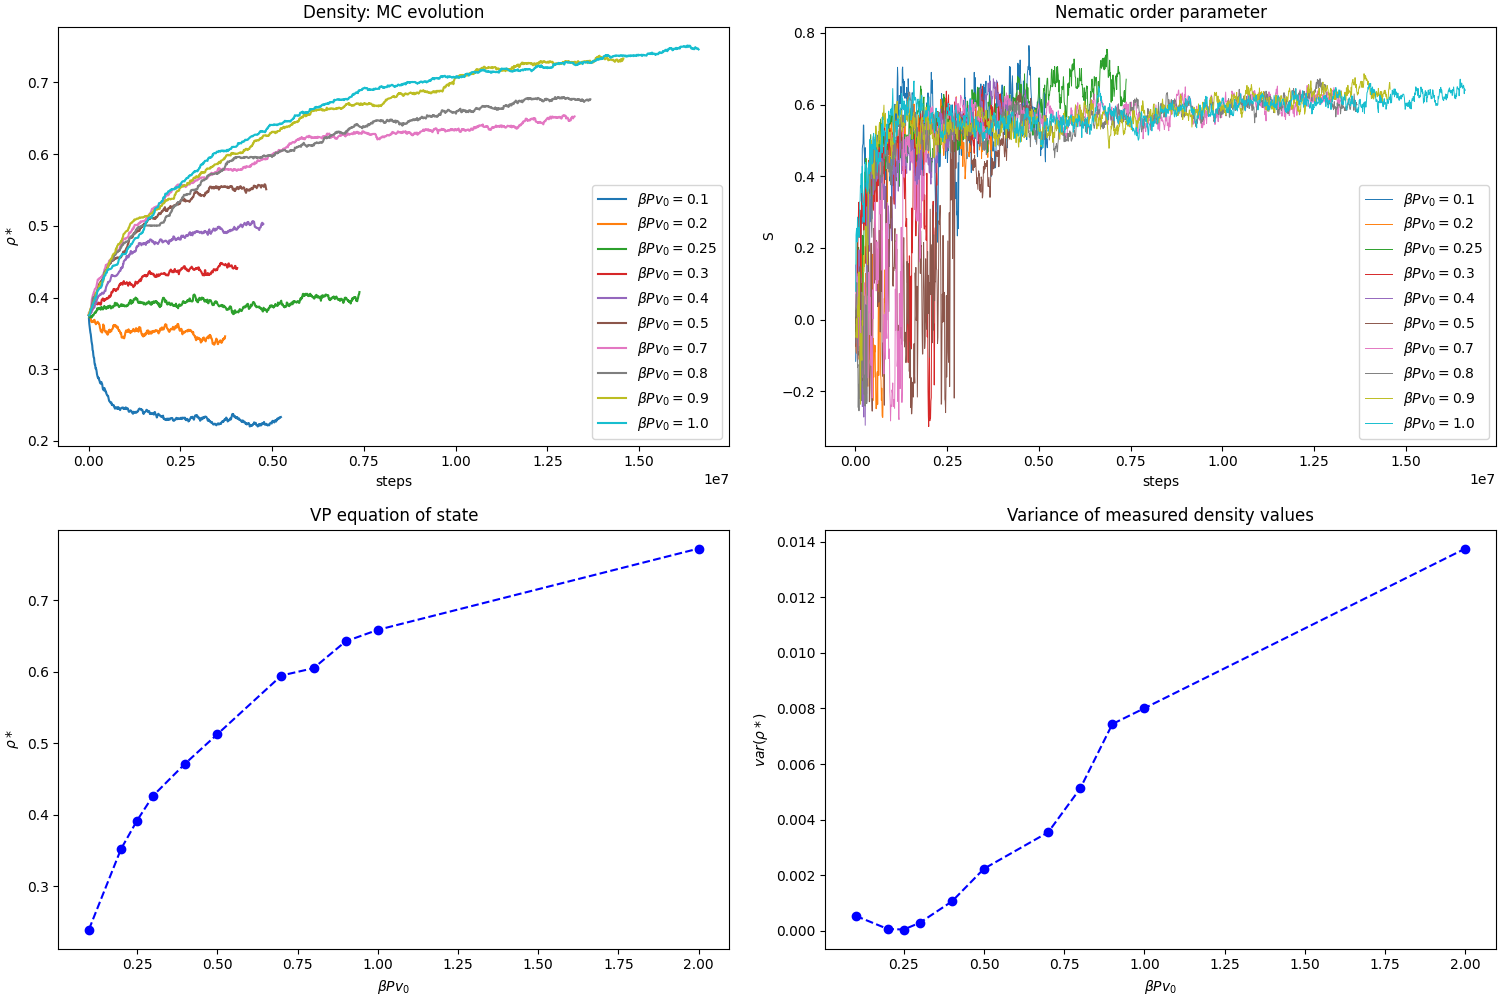
\includegraphics[width=1\textwidth]{/home/hugens/shared/uni/modsim/modsim/project/figures/NPT}
\par\end{centering}
\caption{NPT\label{fig:NPT}}

\end{figure}

\selectlanguage{english}%
\bibliographystyle{plain}
\nocite{*}
\bibliography{hs}
\selectlanguage{british}%

\end{document}
